\graphicspath{ {mainmatter/Jorda_2003/} }
\title*{2003: Sonigraphical Instruments: From FMOL to the reacTable*}
\titlerunning{Sonigraphical Instruments}

\author{Sergi Jord\`{a}}
\authorrunning{Jord\`{a}}


%\institute{Sergi Jord\`{a} \at Music Technology Group, Pompeu Fabra University, Ocata 1, 08003 Barcelona, Spain  \email{sergi.jorda@iua.upf.es}}
%
%
\maketitle

\abstract*{This paper first introduces two previous  software-based music instruments
designed by the author, and analyses the crucial importance of the visual
feedback introduced by their interfaces. A quick taxonomy and analysis of the
visual components in current trends of interactive music software is then 
proposed,  before  introducing  the  reacTable*,  a new project that is
currently under development. The reacTable* is a collaborative music instrument,
aimed both at novices and advanced musicians, which employs computer vision and
tangible interfaces technologies, and pushes  further the visual feedback
interface ideas and techniques aforementioned.
}

\section{Introduction}

For the last ten years, my main area of interest and research has focused around
the possibilities for bringing  new musical creative facilities to non-musicians,
without degrading neither the music potentially producible, nor the users'
interactive experiences and control possibilities. Moreover,  and  because of my
penchant for free-jazz and improvisation,  I have chosen to concentrate on
real-time interactive solutions,  which I also feel  can  be  more  suitable 
(i.e.  more  easily  encouraging, exciting and rewarding) for the non-musicians
than the more thought demanding non-real-time compositional tools.

New musical tools or instruments designed for trained musicians, or even for
specific performers, can be quite complex and challenging;  as a counterpart 
they  may offer a great amount of creative freedom and control possibilities  t o
their players. On the other hand, instruments designed for amateur musicians or
for public audiences in interactive sound installations, tend to be quite
simple, trying in the best case, to bring the illusion  of control  and
interaction  to their users, while still producing ``satisfactory'' outputs. 
Logically,  these two classes of instruments are often mutually exclusive.
Musicians become easily bored with ``popular'' tools, while casual users get lost
with sophisticated ones. But is this trend compulsory? Wouldn't it  be possible 
to  design  instruments that  can  appeal  to   both   sectors:   tools   that  
like   many traditional acoustical instruments, can  offer  a  \textit{low entry  fee
with no ceiling  on  virtuosity} \cite{Wessel:2001}?  With these  questions  in mind I started
in 1997 the conception and development of FMOL, a path that has recently taken us
to the reacTable*.

\section {Sonigraphical Preliminaries}


\subsection{\textit{Epizoo} (1994--1995)}


Several years before FMOL, together with the  visual  artist and performer
Marcel.l\'{\i} Ant\'{u}nez I had developed the computer-based interactive
performance \textit{Epizoo} (1994--1995).

The project was not a musical instrument; at least not only. Integrating
elements of body  art, video games and multimedia applications, it allowed
volunteers from the audience to  play with (or ``tele-torture'') the  performer's
(i.e. Ant\'{u}nez's) naked body via a graphical interface \cite{Gianetti:1998,Jorda:1996,Lozano-Hemmer:1996}. \textit{Epizoo}'s
graphical interfaces, as seen in Figure~\ref{Jorda:fig:epizoo}, could seem to come from a weird
video game designed by the likes of Hieronymus Bosch or Giuseppe Archimboldo, but 
the  fact is, that  these  GUIs still stick to the typical, hypertextual
multimedia cd-rom or web approach: buttons (albeit very hidden) for discrete
selections, and sliders (or hot-spots that evaluate mouse activity) for
continuous  controllers.

\textit{Epizoo} musical output was mostly  based on wave file loops and MIDI sequences;
loops were often layer-able and pitch-changeable, and sequences could be
sometimes manipulated in several ways, but each of \textit{Epizoo}'s screens (there are
about 15 screens in the complete performance) can be considered  in fact more as
 a  musical piece or  composition, which  happens  to have different
performances every show, than a true musical instrument.  Besides,  volunteers 
did  really  conduct  all  the show  development, including  the  music  and  the
 light show, and they did so through  its quite peculiar mouse-driven GUI, but the
opportunity  to manipulate a real human body  seemed to mask all other ``banal''
interaction possibilities. This, combined with the fact that these users (which
could typically have many different ``mouse-skills'') were being exposed to the
interface for the first time, but were still responsible of conducting a show in
a cathartic atmosphere, closer to a rock concert or  a  techno  rave than  to  a 
\textit{typical} interactive installation, turned \textit{Epizoo} (at least its musical part) into
a perfect example for the category earlier exposed: interactive sound 
installations  which  promote  the  user's  illusion   of control while
guarantying their musical output. Whatever the user did, s/he could feel the
control  over the whole show, but at the same time the output, especially  the
musical one, would never be ``too bad.'' FMOL was not going to be about that.

\begin{figure}[t]
\centering
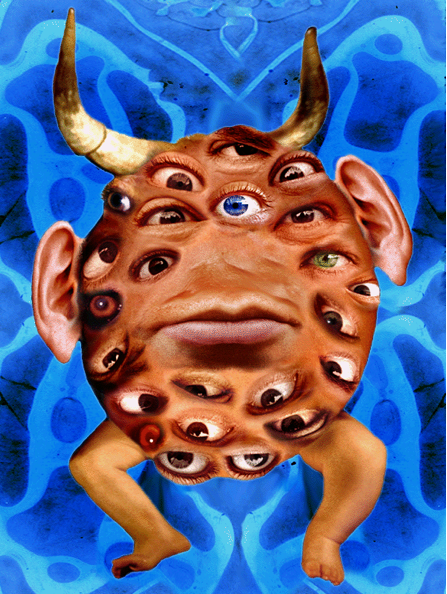
\includegraphics[width=6cm]{Fig1.png}
\caption{In EAX, one of \textit{Epizoo}'s screens, the eyes follow the mouse. The eyes,
mouth, ears and legs are hot spots that can be touched and clicked.}
\label{Jorda:fig:epizoo} 
\end{figure}

\subsection{Reintroducing FMOL (1997--2002)}

FMOL, a project I started in 1997  when the Catalan theatre group La Fura dels
Baus proposed to me the conception and development of an Internet-based music 
composition  system that could allow cyber-composers to participate in the
creation of the music for La Fura's next show, supersedes most of \textit{Epizoo}'s
musical limitations. The FMOL project has  evolved since  its  debut, and 
several articles  have  been  written  that should not be repeated here. The fact
is that FMOL exemplifies several paradigms which can be treated independently. It
is primarily a tool for collaborative  musical composition  on the Internet. This
feature that was the motto of the initial project is better  exposed  in  \cite{Jorda:1999}, 
which  deals  with  the  social  and aesthetic implications of net-music, and
 \cite{Jorda:2001} which cover more technical aspects of the implementation. Furthermore,
implications of computer and web based collective or collaborative  music 
composition  and  performance,  starting with the \textit{League of Automatic Composers} in  the  late  70s  \cite{Bischoff:1978} have been widely studied and published  in these last
years in papers and thesis such as \cite{Barbosa:2002} and \cite{Follmer:2001}.

Technical aspects of the FMOL software (real-time synthesis engine, etc.) are
covered in \cite{Jorda:1998}. The didactical, intuitive and proselytizing aspects of FMOL as a
tool for introducing newcomers into experimental electronic music are deeply
treated in \cite{Jorda:2002}, while \cite{Jorda:2002a} or \cite{Jorda:2002b} also cover its use as a professional  
instrument   and   its    attempt    at    dealing simultaneously   with  
micro-sonic and    macro-musical compositional ideas.

In this paper I want to focus only on the peculiar aspects brought by FMOL's
unique user interface, which presents a closed feedback loop between the sound
and the graphics: in FMOL, the same GUI works both as the input for sound  control and as an output that intuitively displays  all  the  sound  and music activity. After explaining
deeper this idea, I will discuss different ways where these sonic-graphic
relations are present in recent audiovisual software, and the path that has led
us to the conception of our new project, the reacTable*.

\subsection{FMOL Musical Output}

With FMOL I wanted to introduce newcomers to experimental electronic music
making. Therefore, for obvious availability reasons,  the instrument  had to be a
mouse-driven software (it can still be  freely  downloaded  at  \cite{Jorda:2002}).  I  also
wanted to create a simple and complex tool  all at once; a tool that would not
dishearten hobbyist musicians, but would still be able to produce completely
diverse music, allowing a rich and intricate control  and  offering  various 
stages of training and different learning curves.

Both goals have been, in my opinion, quite well attained. During the two
Internet calls for musical contributions  for two of La Fura's shows
(January-April 1998 for F@ust 3.0, and September-October 2000  for the opera DQ)
more than  1,700 compositions were received in the database. We know now
that many of the participants had no prior contact with experimental electronic
music and that a few were even composing or playing for the first time, but the
final quality of the contributions (which can be heard online, as well as on the
the Furadels Baus' F@ust 3.0-FMOLCD published in 1998 \cite{Jorda:1999}, and on the more
recent CMJ 2002 companion CD \cite{CMJ:2002}) was quite impressive.

Moreover, I have given several  FMOL workshops  usually with a mix of
musicians and non-musicians,  and if the feeling is positive they usually end
with public concerts. An improvisation fragment recorded after one of these
workshops can also be heard in the CMJ CD \cite{CMJ:2002}. The intuitiveness acid test took place in
March 2003 during a one-day workshop with 5 to 8-year old kids from Galicia
(Spain), which ended with surprising collective  improvisations.

It takes about half-hour to start having fun with the instrument, and several
hours  to acquire some confidence and produce controllable results. However,
after five years of playing it, I am still  learning it and do often discover
hidden features.  Because,  and  that  is  another  important  point,  it
happens that the instrument I originally designed as  a cheap and freely
available system for ``experimental electronic music proselytism,'' turned to be,
to my own surprise, my favorite instrument for live concerts. Since 1999, the
FMOL Trio (Cristina Casanova and me on FMOL computers, plus Pelayo F.
Arrizabalaga on saxophones/bass clarinet and turntables) performs free-form
improvised electronic music and has produced several live CDs \cite{Feller:2002,Trio:2000,Trio:2002,Trio:2002a}.

\subsection{FMOL Visual Feedback}

Arguably, visual feedback is not very important  for playing traditional 
instruments,  as   the   list   of   first   rank   blind musicians and
instrumentalists (e.g. Ray Charles, Roland Kirk, Tete Montoliu, Joaqu\'{\i}n
Rodrigo, Stevie Wonder \ldots{}) may suggest. But traditional instruments usually
bring  other kinds of feedback, like haptic  feedback \cite{Bongers:1994,Gillespie:1999}, which is 
not  so often  present  in  digital  instruments, at  least  in  the  ``cheap''
ones. Besides, why should not digital  instruments  use at their advantage
anything that could broaden the communication channel with its player? I am
convinced that in the case of FMOL, its unique visual feedback has been a
fundamental component for its success as a powerful and at the same time
intuitive and enjoyable instrument.

FMOL mouse-controlled GUI is so tightly related to the synthesis engine 
architecture, that almost every feature of the synthesizer is reflected in a symbolic, dynamic and non-technical way in the interface. In  its  rest position  the  screen looks like a simple 6x6 grid or lattice. Each of the six vertical lines is associated with  one  voice  generator (FMOL's sound engine supports six real-time synthesized stereo audio tracks or channels), while the horizontal lines are associated  with the effects processors
(filters, reverbs, delays, resonators, frequency, amplitude  or ring  modulators,
 etc.), embedded  in each track. All of these lines work both as input devices
(controllers) that can be picked and dragged with  the  mouse, and as output
devices that give dynamic visual and ``sonic'' feedback.

\begin{figure}[t]
\centering
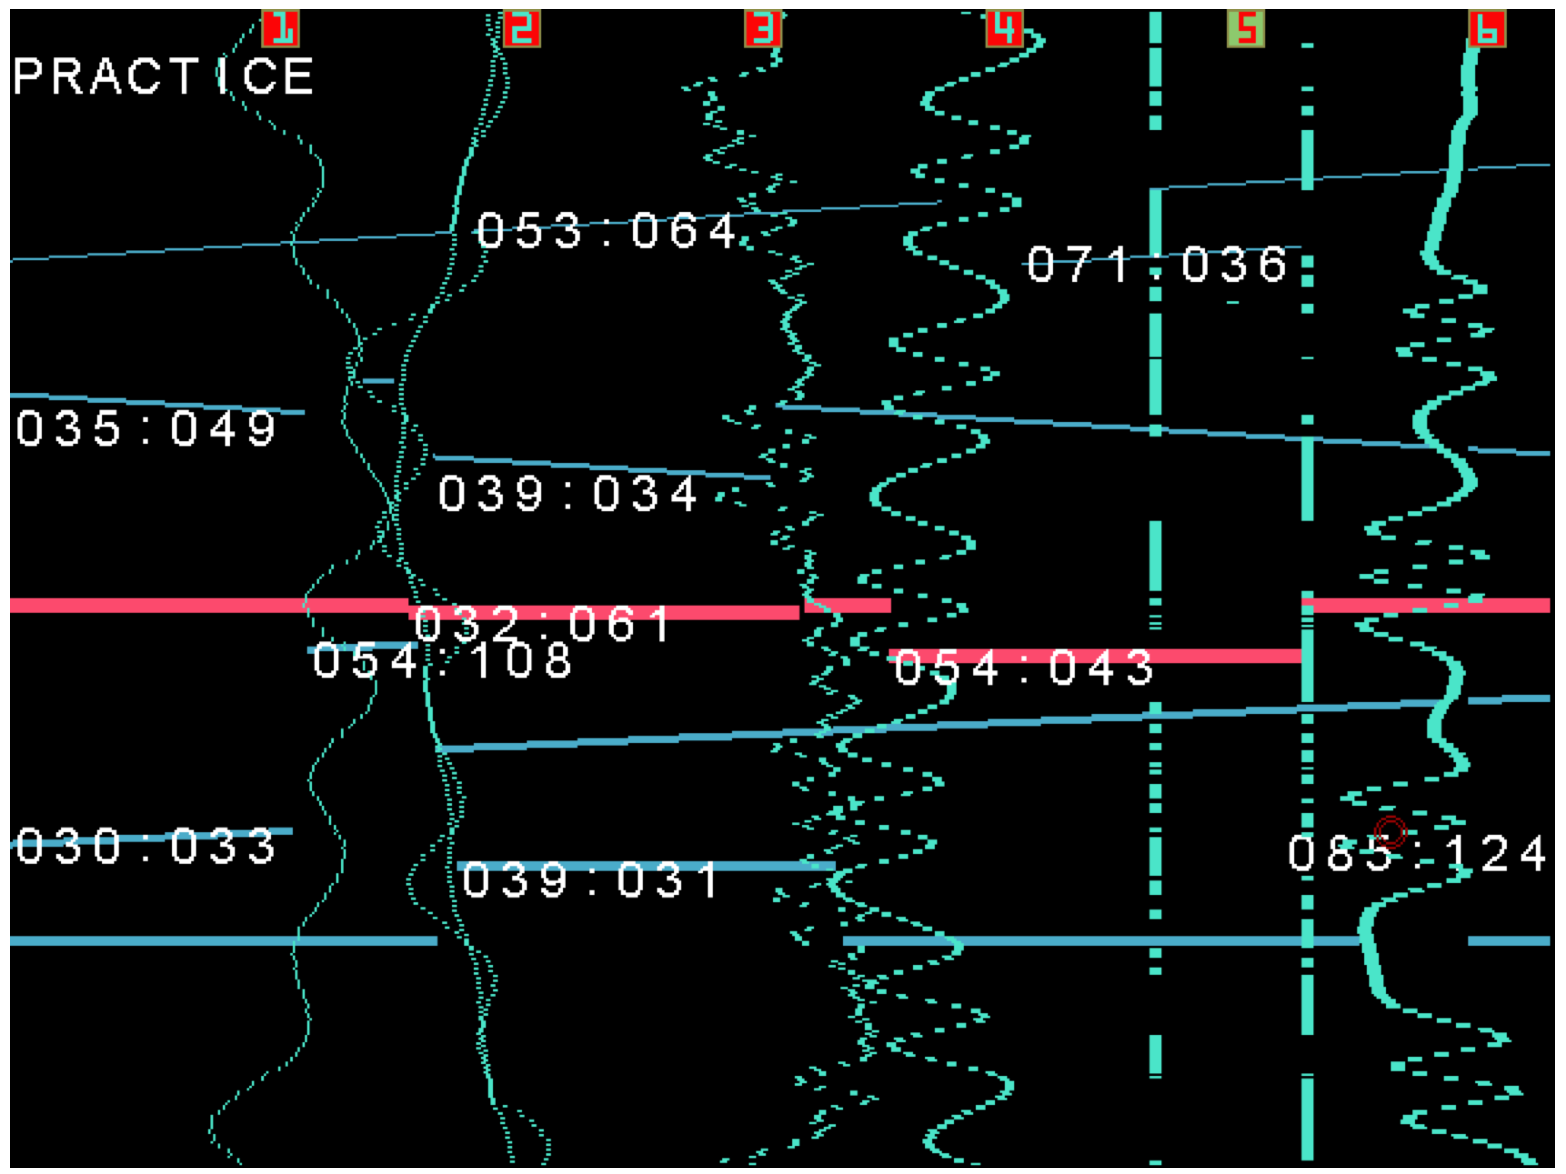
\includegraphics[width=9cm]{jorda-fig2.png}
\caption{FMOL in action.}
\label{Jorda:fig:fmol} 
\end{figure}

Mappings and detailed control mechanisms are explained better in \cite{Jorda:2002}. The key
point  is that when multiple  oscillators or segments are active (FMOL engine
includes 24 LFOs and 96 parameters to control), the resulting geometric
``dance,'' combined  with  the   six-channel  oscilloscope information given by
the strings, tightly reflects the temporal activity  and intensity of the piece
and gives multidimensional  cues to the player. Looking at a screen like Figure~\ref{Jorda:fig:fmol}
(which is taken from a quite dense FMOL fragment), the player can intuitively
feel the loudness, frequency  and  timbrical  content  of every channel, the
amount of different applied effects, and the activity of each of the 24 LFOs.
Besides, no indirection is  needed  to  modify any of these parameters, as
anything in the screen behaves simultaneously as an output and as an input.

\section{Sonigraphical Tools}

\subsection{Media players and VJ Tools}

In order to show the secular catacomb stage of visual  music, Bernard Klein
affirmed in his 1927 book  \textit{Color-Music:  the Art of Light} that ``it is an odd
fact that almost everyone who develops a color-organ is under the misapprehension
that  he or she, is the first mortal to attempt to do so'' \cite{Klein:1927}. This assessment
could surely not be pronounced anymore nowadays.  While  since  its  beginning, 
digital  technologies have boosted multimodality and any kind of parallelism
between image and sound in any of  their  two directions,  the truth is that in
the last few years, we have seen the flourishing of many software programs or
environments that deal with this duality in several ways, even creating
distinct families of tools each with its well defined idiosyncrasy.

Following the trend started with the popular music visualization freeware
program \textit{Cthugha} released around 1994 and described  on  its  birth  as \textit{an 
oscilloscope  on  acid}, current software  music  players,  like  \textit{WinAmp} or 
\textit{MS Media Player}, come with dozens of fancy visualization  plug-ins,  that allow  the  user  to  view  the  results  of  the  music  in  many different ways. These
systems can be generally described with the following scheme.

\begin{figure}[t]
\centering
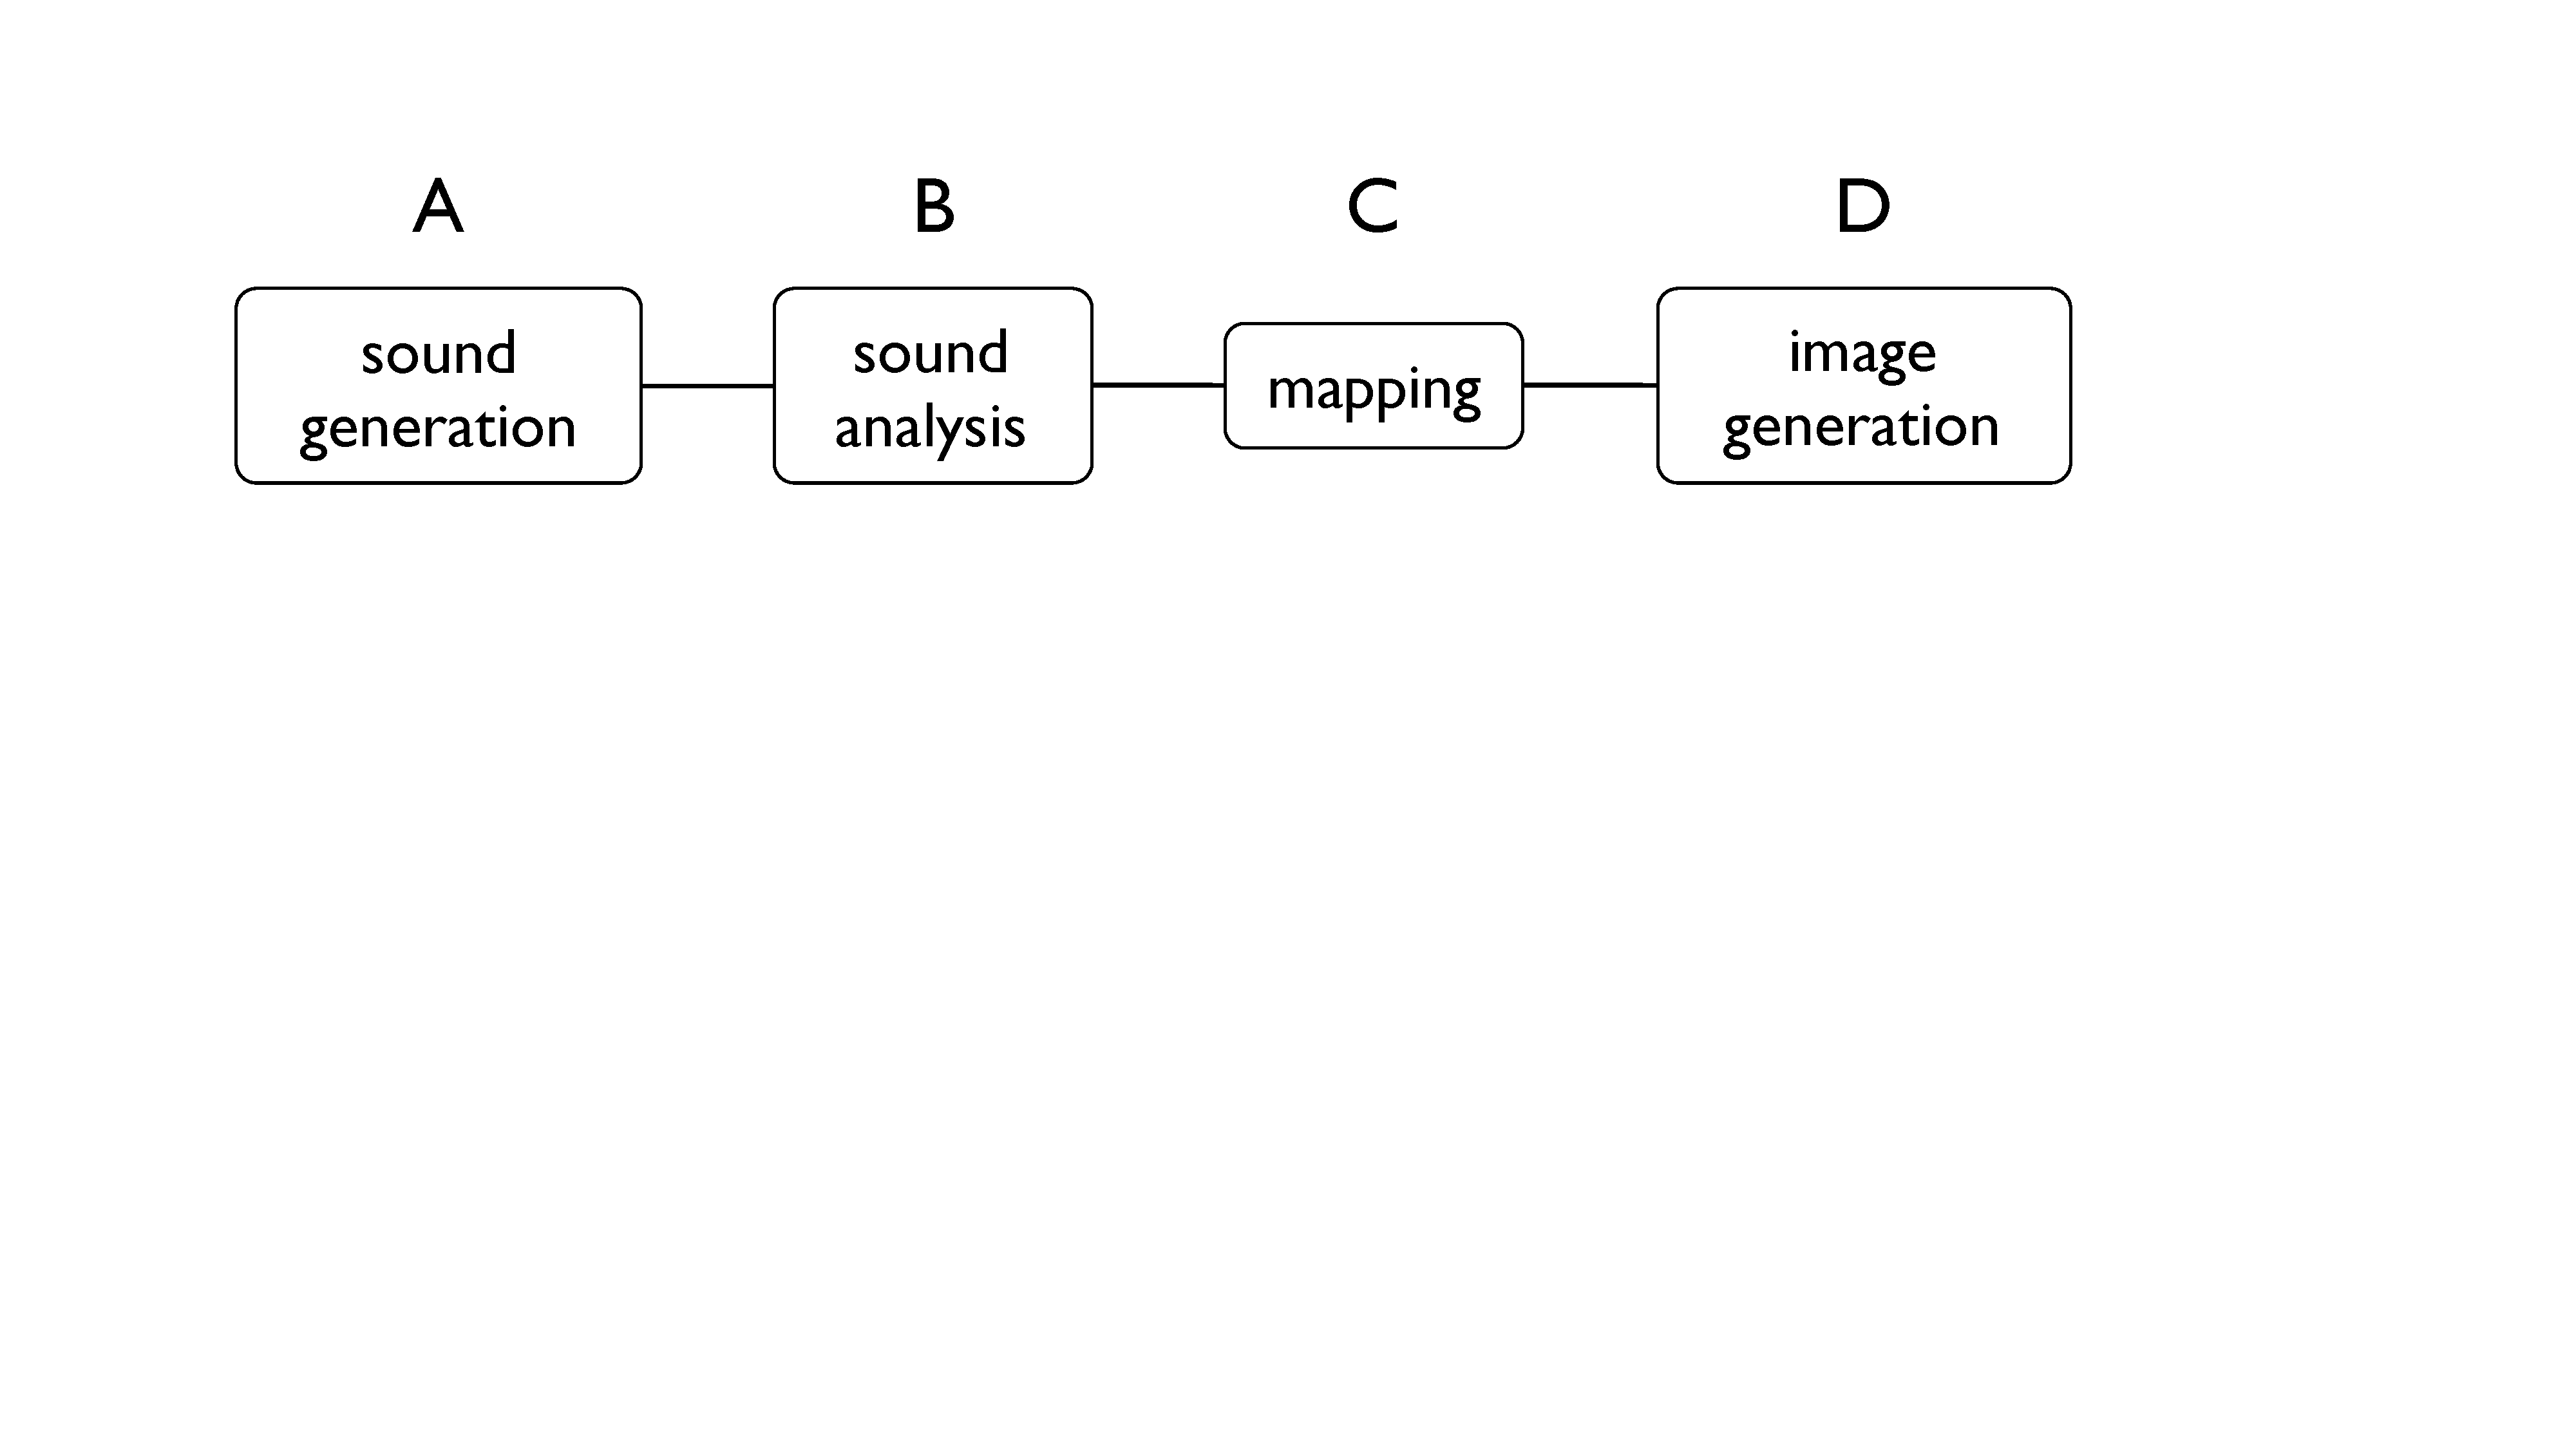
\includegraphics[width=9cm]{jorda-fig3.pdf}
\caption{Elements of a standard music player with visualization.}
\label{Jorda:fig:music-player} 
\end{figure}

However, these systems are not very interactive, except that users can decide to change the visualization  plug-in,  applying thus a discrete change to block D. When an audio-visualizer  of this kind becomes interactive, we have what we could call a VJ Tool. Such tools exist as stand-alone programs such as Jaromil's \textit{FreeJ}, \textit{Arkaos} or \textit{Resolume}, or can be easily  built using  visual  programming  environments  like MAX + (Nato or Jitter), or PD + (GEM or Framestein), to name a few of the more popular software combinations.

In this new case, depending on the particular system design, the user could
interact at any step of the chain.

Using the aforementioned programming environments, one can also decide to take
the complementary approach, and build a musical instrument or a sound
synthesizer which can be directly controlled by the analysis of some dynamic
visuals. These image input can be of  any  kind  (synthetic,  abstract, video,
etc.), and can come from any source (stored movies, real-time generated
animations, live video input, etc.) Although different in concept, this
alternative scheme could also include computer vision based musical controllers.

\begin{figure}[t]
\centering
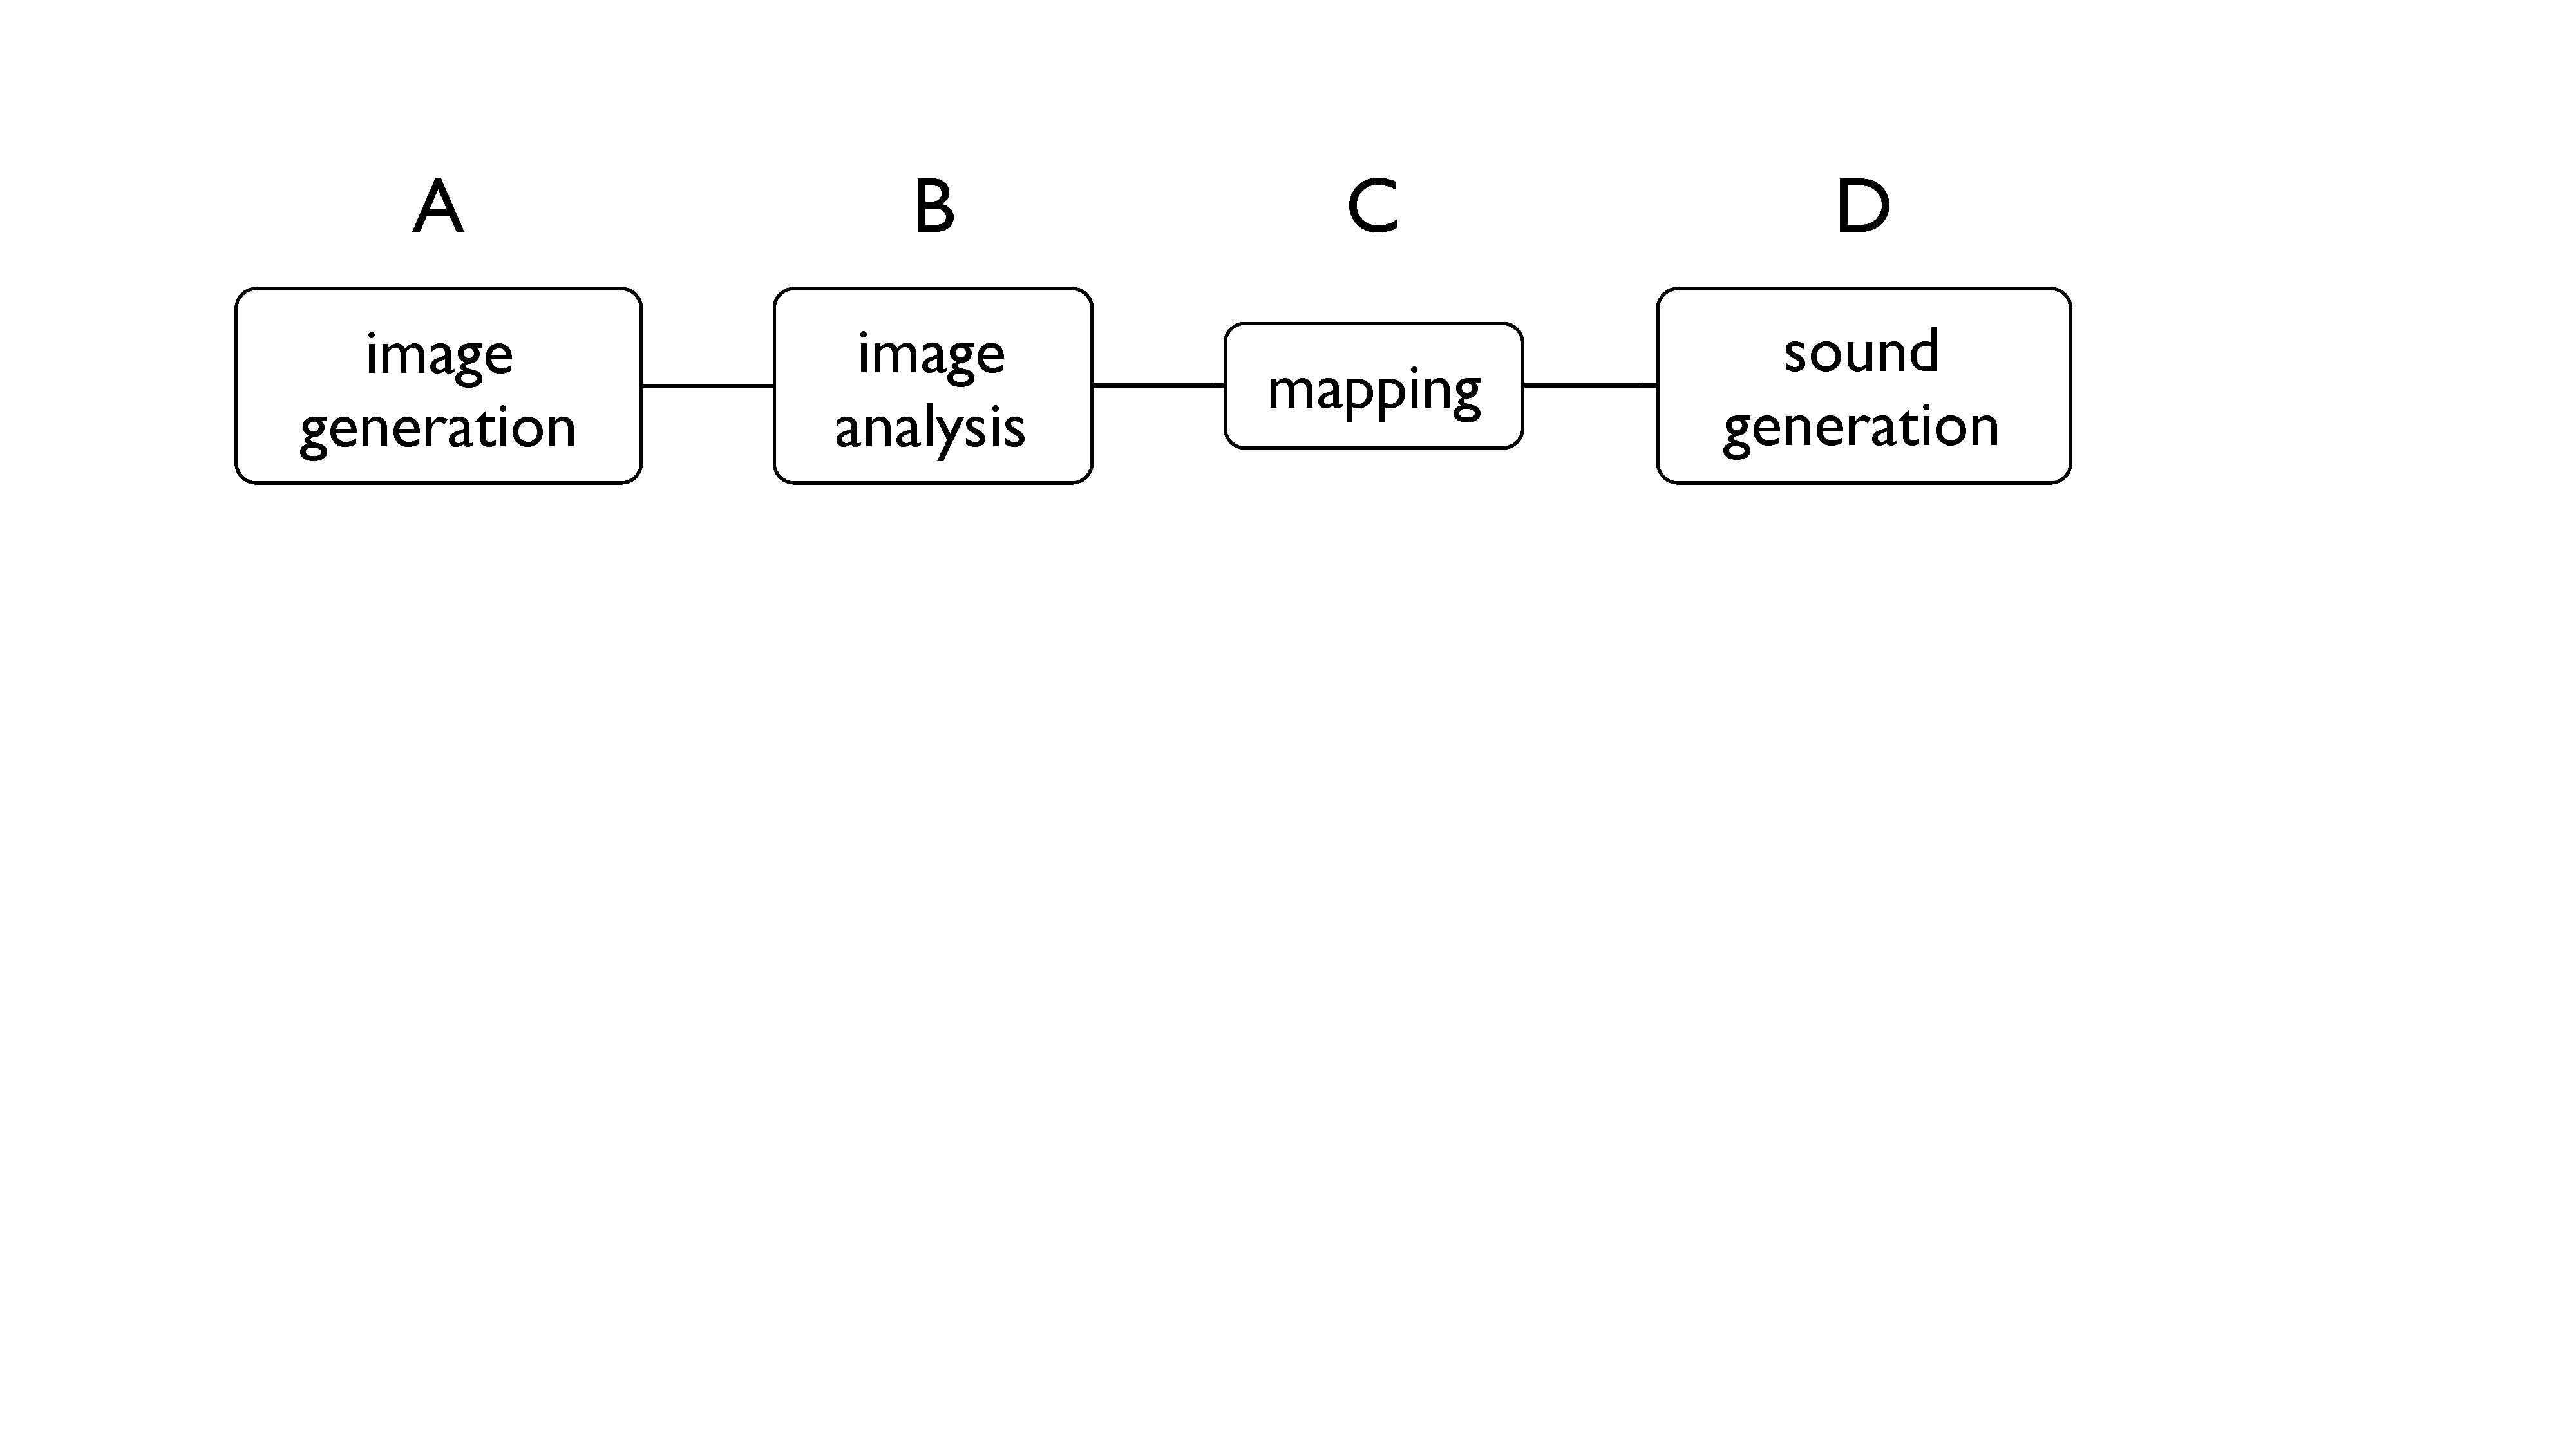
\includegraphics[width=9cm]{jorda-fig4.pdf}
\caption{Elements of an image controlled  music generator.}
\label{Jorda:fig:generator} 
\end{figure}

However, neither of these two approaches (Sound $\rightarrow$ Visuals  or Visuals
$\rightarrow$ Sound)  generally  closes  the  control  loop  as FMOL does
(i.e. in VJ tools, the way the user modifies the graphics does not affect the
music). Besides, they usually present two  windows  at least:  one  for the 
visual  output  (or input, depending on the chosen approach)  and  an additional
one (the ``control panel'') for parameter modification; they do not allow to
modify the \textit{visuals window} by playing directly on it.

\subsection{Golan Levin's Work}

To my knowledge, only Golan Levin's work follows an audiovisual approach
comparable to the one I've presented in FMOL. The fact is that  although  we
unfortunately  did not know about each other until quite recently, I believe
our goals and approaches share many common aspects.  In  his  master thesis
``Painterly Interfaces for Audiovisual Performance'' he proposes a system for the
creation and performance of dynamic imagery and sound, simultaneously, in
real-time, and with basic principles of operation easy to deduce, while at the
same time capable of sophisticated expressions and indefinitely master-able \cite{Levin:2000}.

\begin{figure}[t]
\centering
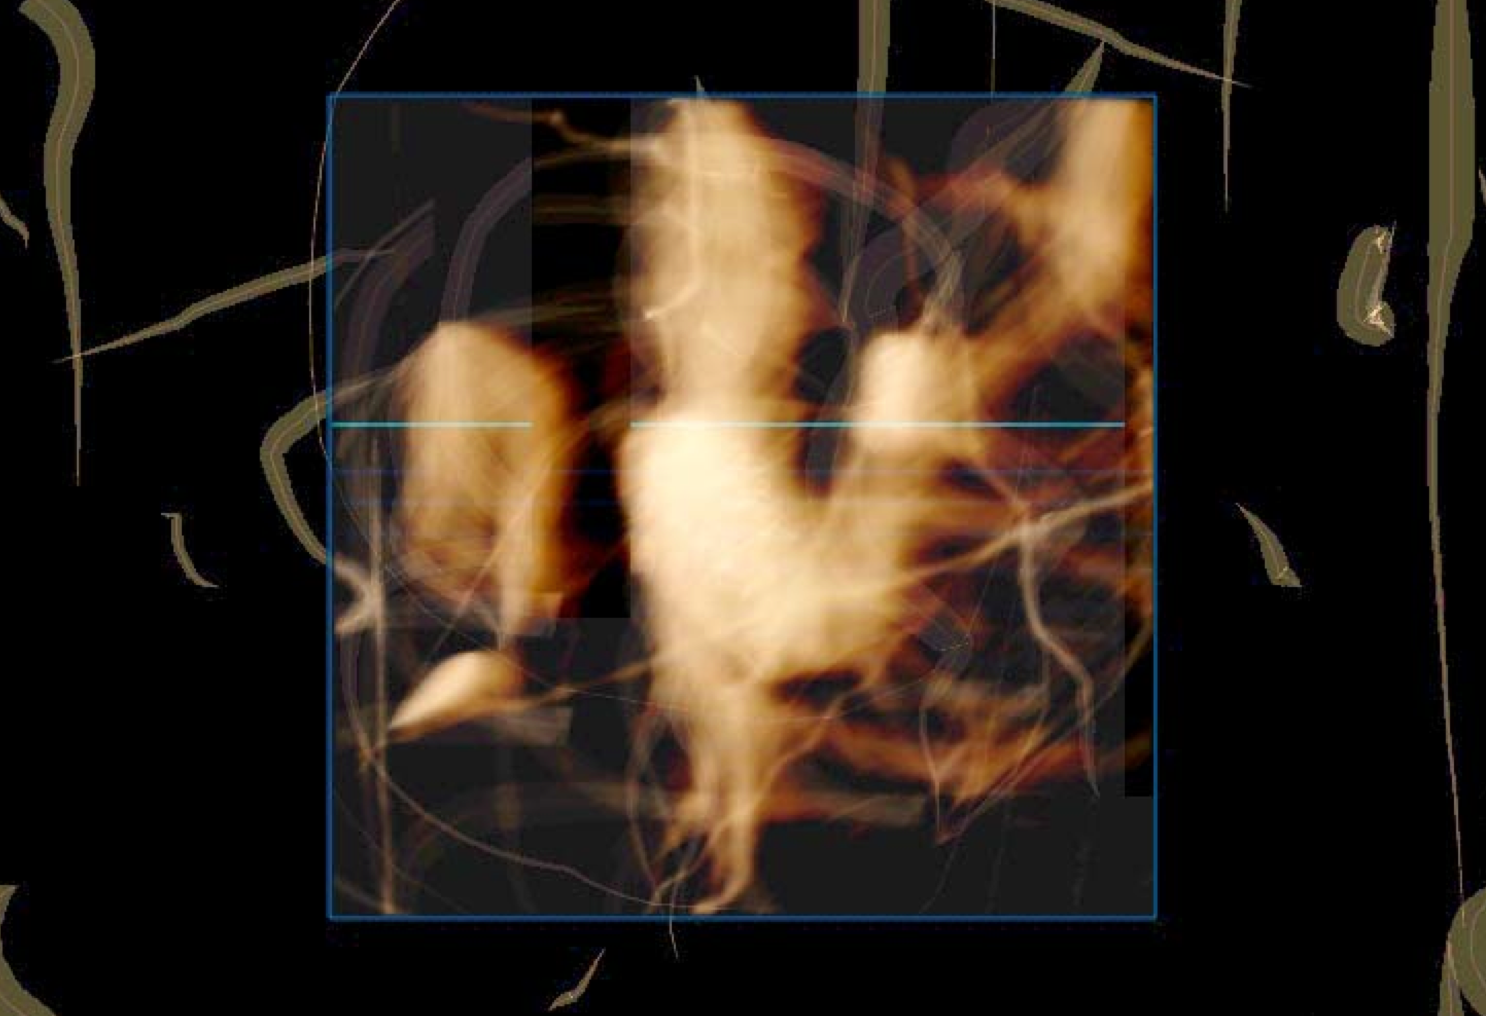
\includegraphics[width=9cm]{jorda-fig5.png}
\caption{A screenshot  of Golan Levin's Yellowtail.}
\label{Jorda:fig:yellowtail} 
\end{figure}

Levin talks about an inexhaustible, extremely variable, dynamic, audiovisual
substance that can be freely painted, and he  has  developed  many  audiovisual  
tools,  like  \textit{Yellotail}, \textit{Loom}, \textit{Warbo}, \textit{Aurora},  and  \textit{Floo}, which  follow  this  path. Perhaps, the major difference in our approaches may be the fact that Levin, like Oskar Fischinger, the animator that in the 40s invented the \textit{Lumigraph} color organ \cite{Moritz:1997}, is willing to play light while playing sound.  For him, image is therefore an end in itself. While for me, it is only  the means to an end: a
more intuitive interface for creating music.

\section{The reacTable*}

\subsection{Preliminary}

Last year, together with the doctorate students  Alvaro Barbosa,    Gunter   
Geiger,    Rub\'{e}n    Hinojosa,    Martin Kaltenbrunner and Jos\'{e} Lozano,
and the  undergraduate students Carlos Manias and Xavier Rubio, we constituted
the Interactive Systems Team, inside the Music Technology Group led by Xavier
Serra at the Pompeu Fabra University of Barcelona. One of the initial projects
was to port FMOL  to Linux and make it open-source, which seemed also a good
opportunity for revamping the system.

Looking at the way people have used  FMOL, and  using  it myself for
improvisation in different contexts and with different musicians, has raised
ideas new features and modifications. But we also felt that  this  control 
complexity could not be permanently increased; there  are limits  to  what can be
efficiently achieved in real-time by means of  a mouse and a computer keyboard.
Building an external FMOL controller for a faster and more precise
multi-parametric control seemed therefore a tempting idea. Designing  a video
detection or ultrasound system that would  allow musicians  to  interact on a big
projection  screen, grabbing  and moving  strings  with their hands, was the
first idea we had. This could surely add a lot of visual impact to live concerts,
although we also felt that musical control and performance may not necessarily
improve with it. These and other considerations took us to a completely new path,
which should profit  the  knowledge  gained  during this years and bring it to a
much more ambitious  project: The reacTable*.

\subsection{Intentions}

We aim at the creation of a state-of-the-art interactive music instrument, which
should be collaborative (off and on-line), intuitive   ( zero manual,   zero instructions),   sonically challenging and interesting, learnable, suitable for
complete novices (in installations), suitable for advanced electronic musicians
(in concerts) and  totally  controllable  (no  random, no hidden presets\ldots{}). The reacTable*  should  use  no  mouse, no keyboard,  no  cables,  no  wearables.  It  should   allow  a flexible number of users, and these should  be able to enter or leave the  instrument installation   without previous announcements. The technology involved should be, in one word, completely transparent.

\subsection{Computer Vision and Tangible  Objects}

As the Tangible Media Group directed by Professor Hiroshi Ishii at the
MIT Media Lab states, ``People have developed sophisticated skills for sensing 
and  manipulating our physical environments. However, most of these skills are  not employed by traditional GUI\ldots{}. The goal is to change the \textit{painted bits}
of GUIs to \textit{tangible  bits}, taking  advantage of the richness of multimodal human
senses and skills developed through our lifetime of interaction with the physical
world.'' \cite{Ishii:1997}.  Several  tangible  systems  have  been  constructed based on
this philosophy. Some for musical applications,  like \textit{SmallFish}, the 
\textit{Jam-O-Drum} \cite{Blaine:2000,Blaine:2002}, the  \textit{Musical Trinkets} \cite{Paradiso:2000a}, \textit{Augmented Groove} \cite{Poupyrev:2000} or the \textit{Audiopad} \cite{Patten:2002}, but we believe that no one attempts the level of integration, power and flexibility we propose.

\begin{equation*}
\texttt{reacTable* = FMOL + MAX + Jam-O-Drum}
\end{equation*}

Substitute if  you  want  \textit{MAX} with \textit{PD} or \textit{JMax} or  even \textit{AudioMulch}. Substitute the \textit{Jam-O-Drum} with the table version of \textit{Small Fish}. You can even substitute FMOL, but only  with Levin's systems, and you will get an initial idea about what the reacTable* is all about:  a table-based collaborative  music instrument that uses computer vision and  tangible user interfaces technologies, within a MAX-like architecture  and scheduler, and with FMOL-inspired HCI models and visual feedback.

The reacTable* is a musical instrument based  on  a round table,  which  has  no
 sensors,  no  cables,  no   graphics  or drawings. A video camera permanently
analyses the surface of the table, while a projector draws a dynamic and
interactive interface on it.

Many interesting and promising computer vision tools, mostly based on body
motion capture, are being developed  for musical applications \cite{Camurri:2001,Camurri:2002}. 
However, many of us  do  not feel too comfortable ``dancing'' in front of a
video camera (some even without camera!), while we all work and socialize around
tables. For this reason our computer vision  system  does  not attempt to track
body motion. Instead, it focuses on  tracking the  hand  movements  over  the 
table,  and  on  detecting  the nature, position and orientation of the objects
that are distributed on its surface.

These objects are mostly passive and made out of plastic  or wood of different
shapes. Users interact with them by moving them,  changing  their  orientation 
on   the   table   plane   or changing their faces (in the case of volumetric
objects). More complex  objects  include  (but  are  not  limited  to)  flexible
plastic tubes for continuous multi-parametric control, little wooden dummy
1-octave keyboards, combs (for comb-filters), or other everyday objects. In case
an object needs sensors, its communication with the host computer will be
wireless.

\subsection{Visuals (1)}

The projection  follows  the  objects  on  the  table  wrapping them with auras
or drawing figures on top of them. The projection covers also the  whole table 
surface with dynamic and abstract elements that reflect all the system's
activity, and depend on the hands' movements and trajectories, the objects' types
and positions, and the relations  between them all. The projection never shows buttons or widgets of any kind.

\begin{figure}[t]
\centering
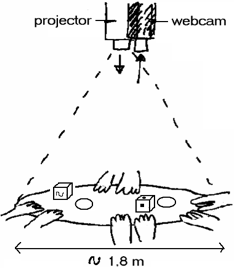
\includegraphics[width=60mm]{Fig6.png}
\caption{The reacTable* simplified scheme.}
\label{Jorda:fig:reactable-simplified} 
\end{figure}


\subsection{But where is MAX?}

FMOL has proven to be quite flexible. Its palette of sound generators and
processors includes  more than  20  algorithms that (with internal configuration 
variations)  constitute a bank of  127  presets the  user  can  select and 
apply to  any  of  the strings. This process of ``building an orchestra'' is not
done in real-time while playing, but in a different, more conventional window.
Besides, all FMOL macro-control of form is done like in traditional analog
synthesizers, by means of LFOs and arpeggiators. More sophisticated control
sources, such as algorithmic generators, pitch filters, etc. cannot fit
coherently into the FMOL interface. The reacTable* overcomes these restrictions
by adapting one of the more powerful real-time computer music software paradigms
implemented in the last decades.

Like  MAX  and  all  of  its  cousins,  the  reacTable* distinguishes between
control and sound objects, and between control and sound  connections.  Unlike 
MAX, and  more like Audiomulch (which however has no explicit  control flux), the
reacTable*  objects are more high-leveled; the  reacTable*  is an ambitious
project but  it  \underline{is} an  instrument, not  a programming language!

When a control flow is established between two objects, a thick straight line is
drawn between them, showing by means of  dynamic animations, the  flux 
direction,  its  rate  and  its intensity. Visual feedback will also guarantee
that LFOs and other  macro-temporal  values  will  be  perceived  as  blinking animations projected on top of the related objects, showing frequency and
shape (e.g. square vs. sinusoidal).

\subsection{Visuals (2): Audio flow}

Where control flow lines are straight and simple, audio flow lines are \textit{organic}
and  complex.  Their  dynamic  shapes  will show the macrotemporal audio
variations (vibratos, tremolos, tempo and rhythms\ldots{}) and their interior
(colors, intensities\ldots{}) will depend on their spectral audio content.

\begin{figure}[t]
\centering
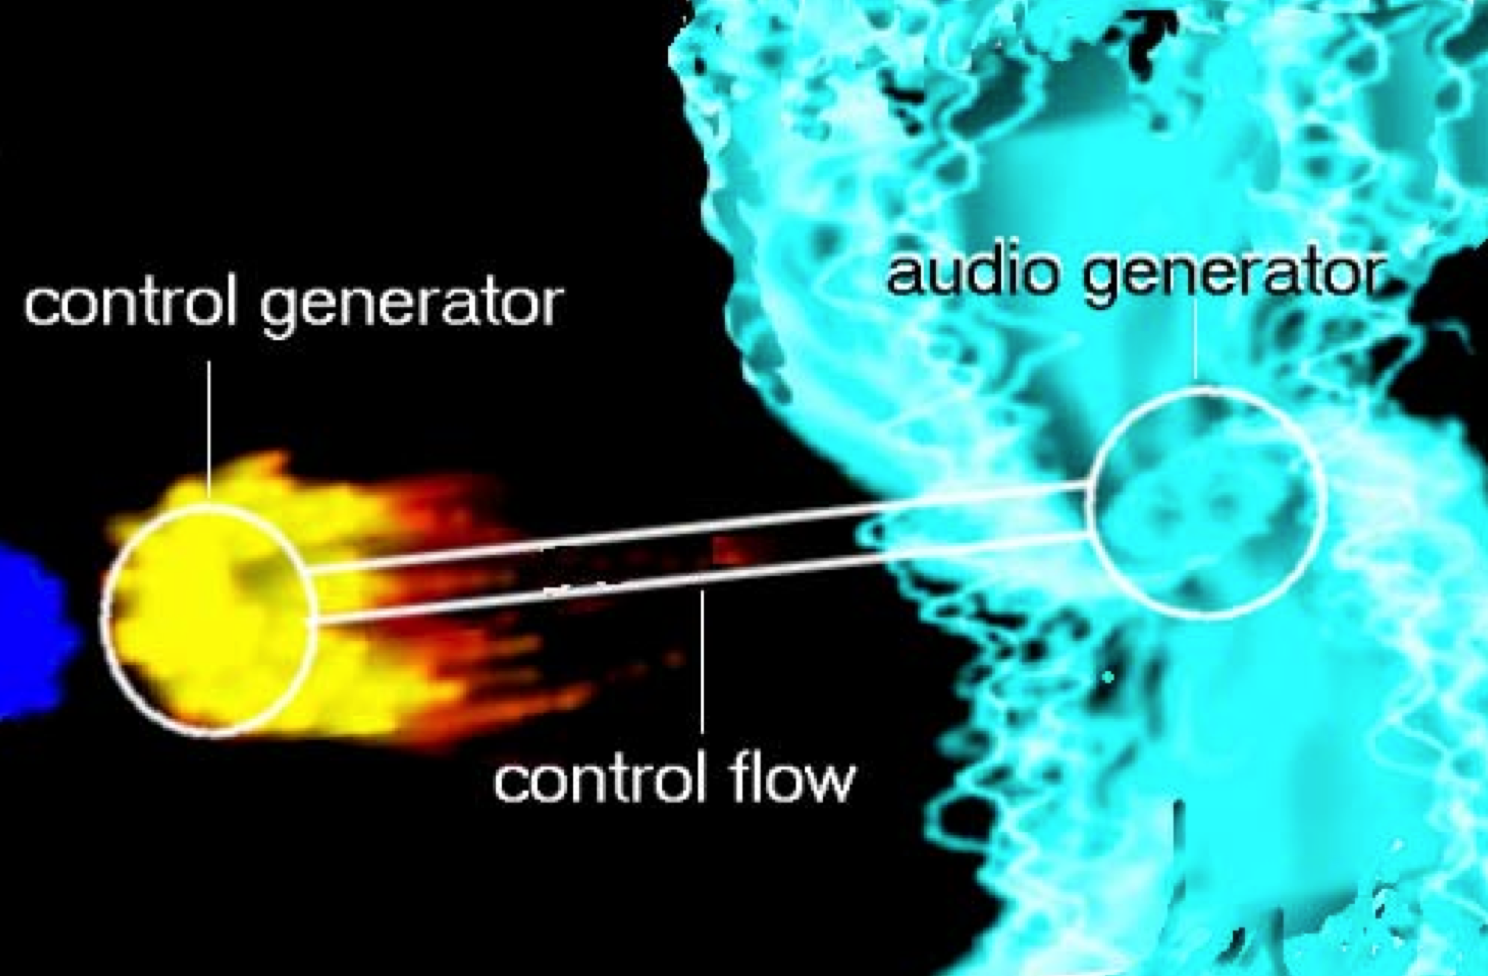
\includegraphics[width=9cm]{jorda-fig7.png}
\caption{Control  and audio flow simulation.}
\label{Jorda:fig:control-audio-flow} 
\end{figure}

Users  will also be able to control, modify or  fork  audio flows  without 
using  additional  objects,  but  just  by  waving their hands, as if they were
digging water channels in the beach sand.

\subsection{Avoid user's frustration at any cost}
To avoid frustrations, a system does not necessarily have to be completely
understandable, but it has to be coherent and responsible. Unlike MAX, the
reacTable* has to work ``by default'' and any gesture has to produce audible
results.  Here are some of its laws:

\begin{itemize}
\item There is not anything like an \textit{editing  mode}
and  \textit{running mode} (at least for \textit{installation  users}); the  reacTable*  is always running and always being edited!
\item Objects are not active until they are touched
\item Active objects have a dynamic visual \textit{aura}
\item Objects are interconnected by proximity
\item If, on  start-up, a  user  activates an  object that  does not sound (e.g. a control  object)  the  closest  audio object is automatically linked to it, and the link is visualized
\item Moving an object on the  table  can change the  relations with the other objects
\item Relations can also be ``fixed'' touching two objects  with the two hands. Fixed links are shown with a thicker line or a different color
\end{itemize}

Perry Cook, in an informal music controllers design decalogue, ironically points
that ``smart instruments are often not smart.'' \cite{Cook:2001}. Although  we
basically  agree with  him, we have come to the conclusion that a system like the
reacTable* must show some kind of intelligent  behavior. For example, as most of
the control objects are adimensional (some, like the dummy keyboard, are not),
when  one  adimensional  control flux is sent to an object that can accept
different inputs, the system chooses what the best parameters to  control  in 
every case are. In another demonstration  of intelligent  behavior, the system
may suggest interesting candidates for a given configuration, by highlighting 
the appropriate objects (in a manner not to be confused with LFOs).

The reacTable*  wants to be  \textit{user-proof}. For  instance,  it seems  natural 
that  after  some  minutes,  people  will  start stressing the system in
different ways, like placing personal objects onto the table. Although it is not
possible  to anticipate all objects  that  people  may use, some of the  more
common could be detected (cigarette packets, mobile phones, keys, pens\ldots{})
and a ``funny'' functionality could be  added  to  them (e.g. mobiles could
generate pitch in a ``mobile-fashion'').

\section  {Current Implementation}

The reacTable* project has started in December 2002 coinciding  with  the 
foundation  of  the  Interactivity  Team within the Music Technology Group (MTG).
We are currently working and researching all the main threads in parallel
(computer vision and objects recognition, sound engine architecture, 
interactivity  logic,  sound  visualization,  etc.) while designing the core and
the integration of all these branches. Computer vision and object recognition is
being carried using both \textit{Eyesweb} \cite{Camurri:1999,Camurri:2000} and the Intel Image Processing (IPL) and Open Computer Vision (OpenCV) libraries.\footnote{\url{http://opencv.org/}} We will
not describe here any of these issues, as we soon plan to devote a whole paper to
them. The synthesis engine is  being  implemented  using  the  CLAM libraries, 
the open-source, multi-platform C++ libraries for real-time audio being developed
at the MTG \cite{Amatriain:2002,Amatriain:2002a}.

In parallel with these two main productions  threads, we are working with a
reacTable* software-only simulator  (that runs on both Linux and Windows), which
is an essential  workbench for defining  and  refining  all  of the  system 
laws, evaluating user interaction and objects' connectivity rules, as well as
determining  the  panoply  of  sound  and  music  objects,  their roles,
behaviors, the way they synchronize between them, etc. The simulator GUI has been
 implemented  in  Java by  Martin Kaltenbrunner, while Gunter Geiger is  working 
on  its  sound engine using PD for quick prototyping. Both modules communicate
via TCP/IP, a flexible architecture which also permits multi-user simulation by 
running  different  instances of the GUI in different computers.

Figure~\ref{Jorda:fig:reactable-simulator} shows  a  reacTable*  simulator  screenshot,  with only four kinds of
sound  objects:  High Frequency Oscillators (circles), Low Frequency Oscillators
(triangles), filters (smoothed squares) and time-based effects (squares). Visual
feedback is yet very simple; all connection lines  are straight and do not
suggest therefore any of the information they transmit, except that to
distinguish between the two types of connections, audio lines are drawn in dark,
while control  lines are light grey. Each dark line  flowing  into  the  audio  sink represented by the black central circle corresponds therefore to an
independent audio thread.

\begin{figure}[t]
\centering
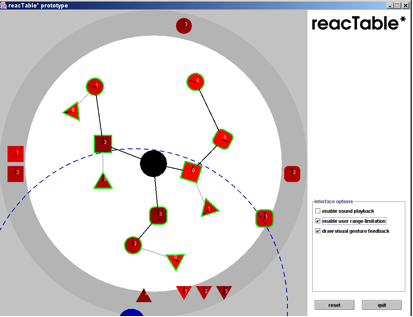
\includegraphics[width=8cm]{Fig8.png}
\caption{reacTable*  simulator snapshot.}
\label{Jorda:fig:reactable-simulator} 
\end{figure}

At this early stage, what we have is  a sort  of higher  level MAX in which
users can drag objects that dynamically interconnect between them according to 
the  rules  defined  in the system. Using the right mouse button objects can
also spin around and connection lines can be broken. Parameters are calculated
from the  rotation angle of  the  objects as  well  as from the length and the orientation of their connections. As simple as it still is, this flexible and dynamic architecture already permits for some fast sound changes that seem impossible to attain in an analog modular synthesizer, which it somehow evokes.

\section {Future Work and Conclusion}

The reacTable*  is an ambitious project. Unlike  many new designed instruments,
its origin does not come from approaching its creation by exploring the
possibilities of a specific technology, nor from the perspective of mimicking a
known instrumental model. The reacTable* comes from our experience designing 
instruments,  making  music  with  them, and listening and watching the way
others have played them. Needless to say, we have deposited a great hope and
expectation on  it.  We  plan  to  have  the  first  integrated  by autumn 2003
and a first full working version by spring 2004.

\begin{acknowledgement}
I would like to thank all the members of the Interactive Systems Team, and
specially  Martin  Kaltenbrunner, for their suggestions on this paper, and Xavier
Serra for his support on this project.
\end{acknowledgement}

\section*{Author commentary: The Genesis of Reactable}
\paragraph{Sergi Jord\`{a}}

2003, the year of the 3\textsuperscript{rd} NIME conference, was also quite an impasse year for me. After graduating in physics in the mid-80s and spending most of the 90s working as a freelance interactive and media artist/designer/programmer, developing interactive installations, performances and music systems (two of them, \textit{Epizoo} and FMOL, had already been introduced in my 2001 NIME paper). With the advent of the millennium I had decided to re-enter academia and pursue a PhD in Computer Music at the Music Technology Group (MTG) founded by Xavier Serra in Barcelona. The MTG was still a very young research group in which the lack of professors or post-docs (Serra was still the only doctor!) was happily compensated with the enthusiasm of everyone, and the most mature PhD candidates shouldered the role of team and project leaders. So here I was, trying to figure out my own PhD thesis, while simultaneously coordinating a team of PhD students that included some of the most talented computer music developers I have ever known. It is within these circumstances that this paper provides an analytical revision of some of my past works and discusses  prospective research directions.

Through the study of the aforementioned examples (\textit{Epizoo} and FMOL), the first half of the paper addresses the potential of what I then called ``sonigraphical instruments,'' a term I coined for referring to instruments in which their GUI acts both as an input for sound control, and as an output that provides a summarized and quickly graspable display of all the sound and music activity. This sonigraphical feature, I argued, is even more pertinent in multithreaded instruments that allow several simultaneous musical processes. These postulates would be furthered in my Phd dissertation published two years later \cite{Jorda:2005}. 

The second half of the paper introduces a multithreaded and sonigraphical DMI, Reactable (known as reacTable* at that time), discussing its main features and the  rationale behind its conception. Considering that this part describes a system that had not yet been tested, not implemented, and in fact, not even fully technically solved, that is, that what it outlines is little more than a personal vision, I now wonder how unlikely it would be that a similar paper would have been accepted in 2015! The presumable different perspectives resultant from this dozen year gap, reflect on one side the maturity currently attained by the NIME field, which was in its infancy in 2003. They could also warn us however about the risks of trying to address too scientifically topics such as the design and evaluation of DMIs, which resist reduction and systematization. For example, although we have published several papers that systemically study the potential benefits of the Reactable in very specific contexts, such as autism \cite{Xambo:2013} or collaboration and peer-learning in public spaces, we have still failed to produce the ``ultimate Reactable-music-instrument evaluation'' paper.

A few months after the publication of this paper, we solved the most crucial pending technical issue and published reacTIVision, an open-source, cross-platform computer vision framework for the tracking of fiducial markers and combined multi-touch finger tracking \cite{Bencina:2005}. Two years later, Reactable was premiered at the ICMC 2005 in Barcelona. It had not been the first musical tabletop; at least the Audiopad \cite{Patten:2002} and the Music Table anticipated it, but it became the more popular one and, arguably,  the most popular DMI to emerge from an academic context. In November 2006 we guilelessly published a video in YouTube, which rapidly and unexpectedly reached millions of views. Three months later, Bj\"{o}rk contacted us and in April 2007 she started touring with a Reactable. Around this same period, the Reactable team also started touring extensively, giving more than 300 concerts, installations and presentations, in 25 countries during the next 3 years. This helped enormously with fine-tuning and improving the system. In 2008 I published what I consider the ``ultimate'' Reactable paper \cite{Jorda:2008}. In 2009, the company Reactable Systems\footnote{\url{http://reactable.com/}} was founded, launching the Reactable Live and the Reactable Experience, and later in 2010, also Reactable Mobile for iOS and Android. 

With Reactable Systems monopolising all the development of the musical instrument, my research shifted towards other areas of tabletop and tangible interaction. It has just recently shifted back to NIME and digital music creation in the shape of ``expert agents for electronic music performance,'' combining research and techniques from musicology, music information research (MIR), machine learning and HCI.\footnote{\url{http://www.giantsteps-project.eu/}} My life has not changed so much, but this 2003 paper set the beginning of a nice story that has not yet ended, and I am definitely happy and proud with what we achieved.

\section*{Expert commentary: Pursuing a Sonigraphical Ideal at the Dawn of the NIME Epoch}
\paragraph{Charles Martin}

A common criticism levelled at the NIME community is that we jump onto the latest available technology, develop one interface, play one concert, send out a paper, and move on. To this criticism, Jord\`{a}'s work on sonigraphical instruments sits as a compelling counter-example.
Jord\`{a}'s paper seems to have appeared at a turning point in his work developing computer-based instruments for collaborative musical interaction, and to be representative of the start of the NIME epoch.

In the first half of his article, Jord\`{a} describes \textit{Epizoo}, a game-like multimedia interface that sits very much in the early-1990s, and FMOL, a collaborative synthesiser running in a late-90s era mouse-driven Windows interface. In the second half, Jord\`{a} outlines the in-progress design for Reactable, a table-top tangible interface that went on to be unveiled through YouTube videos\footnote{\url{https://youtu.be/0h-RhyopUmc}} in 2006 to mainstream acclaim in the tech and music press, and was famously used in Bj\"{o}rk's Volta \cite{Andrews:2007} and Biophilia concert tours starting in 2007. The Reactable could be said to be emblematic of a surge of interest in NIME-research around this time---at least that's when I started to get interested!

So what lessons does this paper hold for the NIME researcher of today?
First of all, this paper shows how perspective and experience acquired through long-term effort in developing musical interfaces is often required for the most interesting designs. The paper itself describes around 10 years of work where Jord\`{a} and his collaborators produced interfaces and invited beginners as well as experienced performers to use them. While Jord\`{a} is satisfied with the utility of FMOL, a successful design by all accounts, years of experience have suggested that there is potential to develop an instrument that is even more intuitive, collaborative, and with fewer compositional assumptions. More than 10 years later, we now know that Reactable achieved these goals, with success as an installation work, as an instrument on the professional concert stage, and with ongoing utility in HCI research \cite{Xambo:2013}. It strikes me as unsurprising that this success should follow a long period of experimentation with different designs, and many different kinds of users.

A second important lesson is Jord\`{a}'s pursuit of a ``sonigraphical'' instrument. In \textit{Epizoo}, FMOL, and in Reactable, Jord\`{a} strives for a kind of unification, or at least colocation, of visual and sonic feedback with the user interface elements. In a sonigraphical instrument, the GUI is ``both an input for sound control, and an output that intuitively displays all the sound and music activity'' \cite{Jorda:2003a}. In FMOL's GUI window, audio signals are visualised in oscilloscope-like waveform traces which can be manipulated with the mouse. In Reactable, the unification is even deeper with a tangible interface projected on a round tabletop. Synth elements are denoted by physical markers which are activated as soon as they are placed on the table. When elements are patched together, oscilloscope traces flow between them to show the signal path. In fact, signal patching and visual connections are unified with physical connection in Reactable, as these are all made simply by moving the markers closer together. Mouse-dragging static patch cords around in Pd or Max feels clunky by comparison!

This level of sonigraphical unity was not achieved without effort on the part of Jord\`{a}'s team. He writes that their first instinct was to develop a system to control a large visual display with body motions. Such an idea would have had similar technological challenges, but none of the intuitive impact and musical possibilities of their final design. The problem of achieving effective sonigraphical designs still challenges NIME-creators today. While mobile multitouch devices would seem to suggest more expressive, tactile manipulation of sound, conservative software continues to be modelled after physical studio setups and antique DAW designs where the primary visual feedback is a VU meter. In 2003, Jord\`{a} defined a benchmark for connections between the sonic, the visual, and the physical in an interface that will amplify the musical intentions of users and minimise frustrations. 
It is notable in Jord\`{a}'s paper that the technical details of his systems are downplayed in favour of explaining the evolution of the sonigraphical design rationale over years of performances and workshops. This, and the success of the Reactable system since NIME 2003, shows us that in NIME research, sustained engagement with performance and users can outweigh short-term technical novelty.

